\chapter{AF}
\label{chap:salvo}
\section{Problem}

% motivation
% explain fluro method
% explain skin model
% explain nelder mead
% explain filter choice

% results in "2d" 
% results in 3d + higher
% future work


\section{Nelder-Mead method}

\begin{figure}[!htbp]
    \centering
    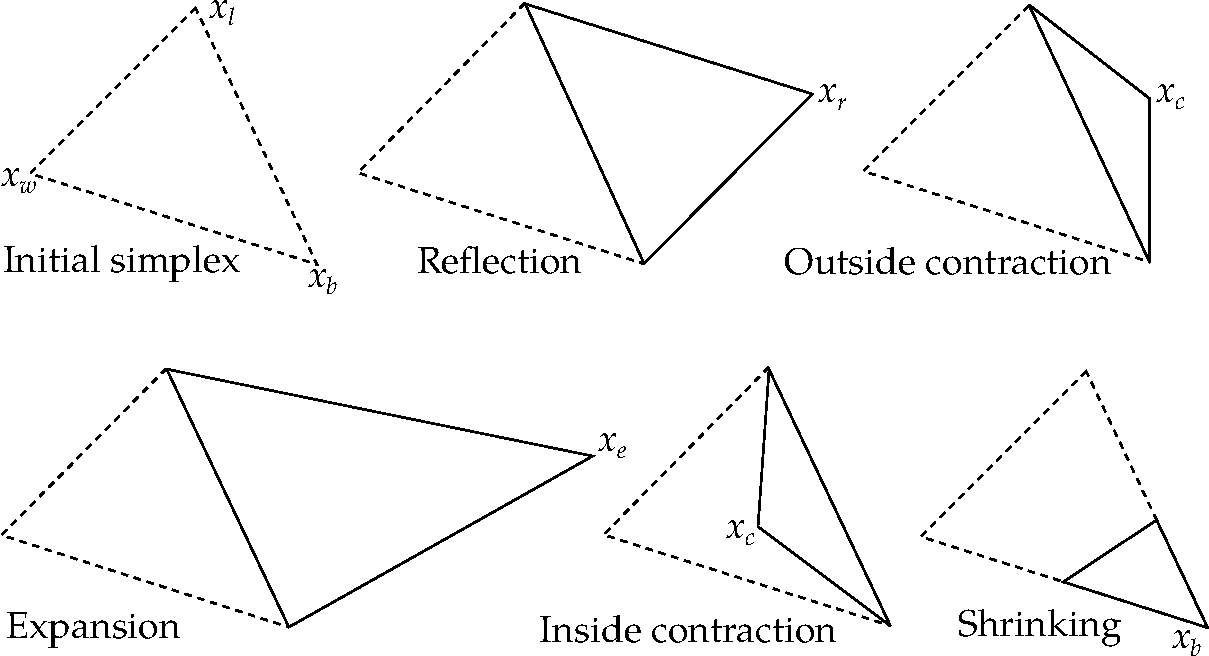
\includegraphics[width=0.75\textwidth]{simplex-operations.pdf}
    \caption{Operations that can be preformed on a simplex for $n=2$.}
    \label{fig:NM-operations}
\end{figure}

\begin{figure}[!htbp]
    \centering
    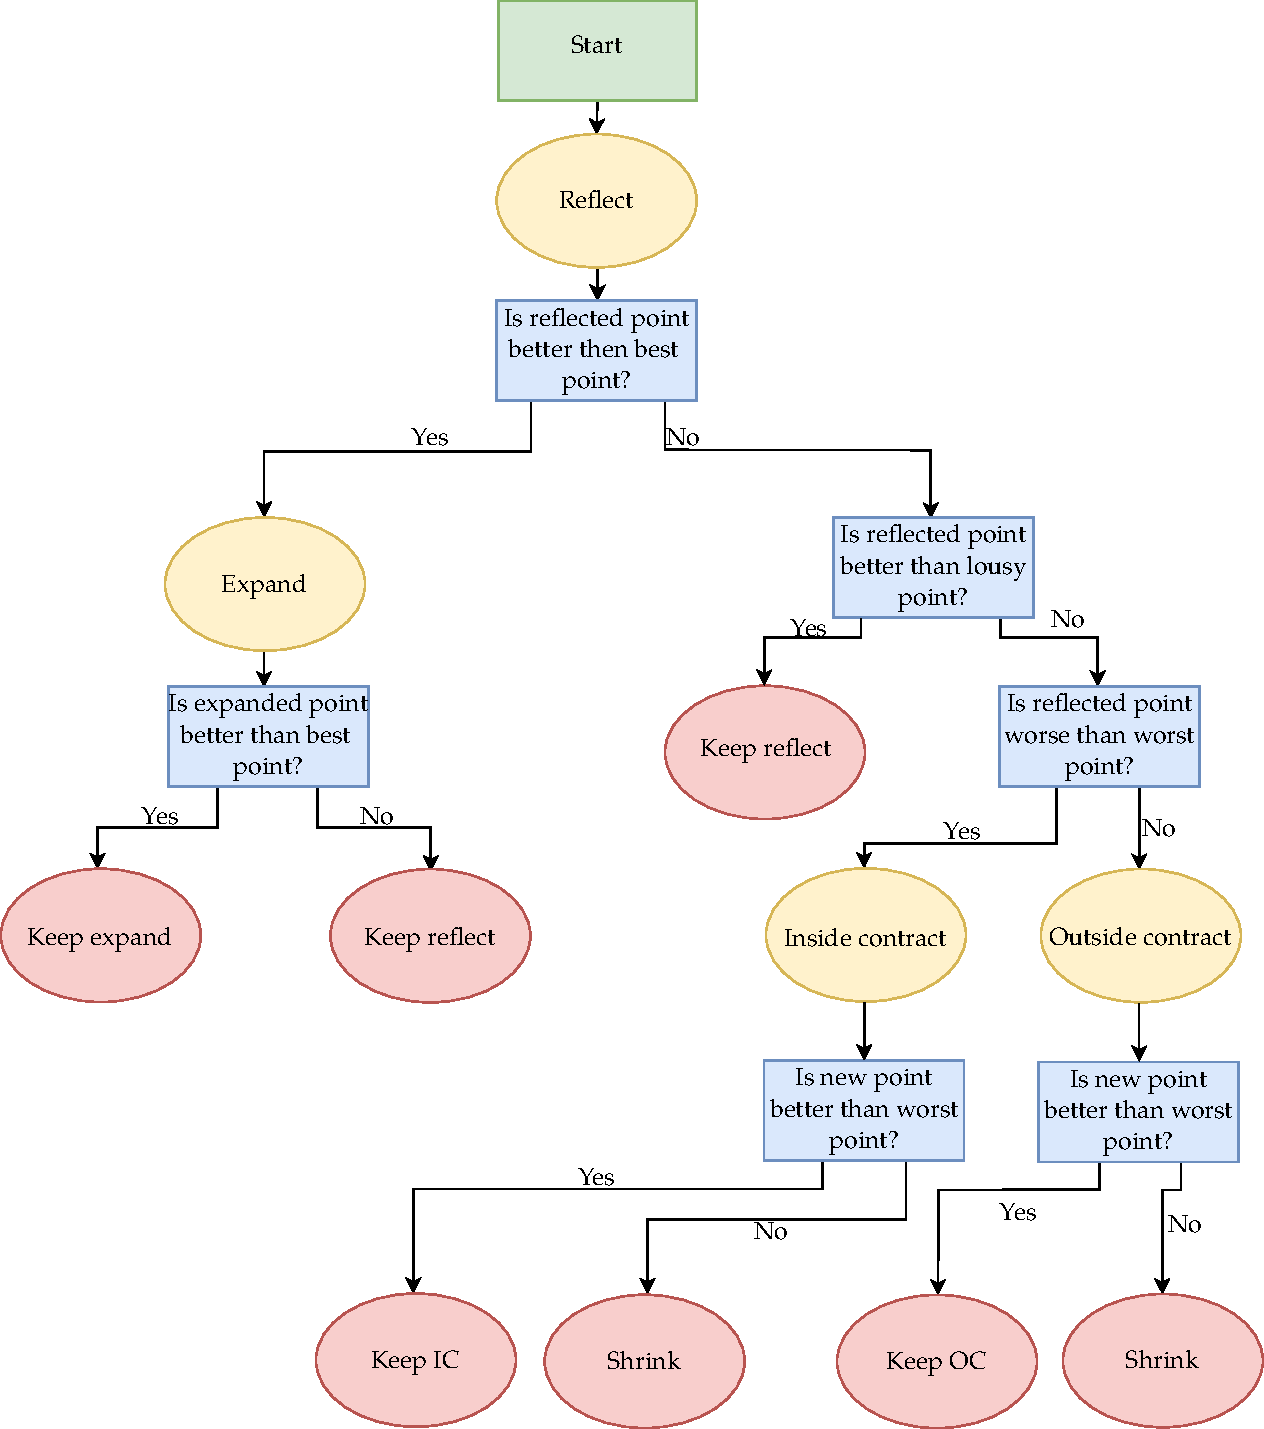
\includegraphics[width=0.5\textwidth]{flowchart.pdf}
    \caption{Nelder-Mead decision tree}
    \label{fig:NM-algo}
\end{figure}




Define $x_w$ as the worst point, $x_l$ and the lousy point, and $x_b$ the best point, such that $f(x_b)\leq f(x_l)\leq f(x_w)$, where $f(x)$ is evaluating the `fitness' of a point.

\begin{align}
c &= \frac{1}{n}\sum \limits_{i=1,i\neq w}^{n+1} x_i \label{eqn:centroid}\\
x_r &= c + \alpha(c - x_w)\label{eqn:reflect}\\
x_e &= c + \gamma(x_r - c)\label{eqn:expand}\\
x_{oc} &= c + \beta(x_r - c)\label{eqn:outsidecontract}\\
x_{ic} &= c + \beta(x_w - c)\label{eqn:insidecontract}
\end{align}

Where $\alpha$ is the reflection coefficient, $\gamma$ is the expansion coefficient, and $\beta$ is the contraction coefficient.



%AF Code works, tested against toy model, may need further validation. 

%No paper or aim for project. Need contact with Dundee/Ninewells to proceed.

\section{Validation}
\section{Practical application}
\section{Conclusion}